\documentclass[a3paper]{article}

% 300 DPI

\usepackage{listings}
\usepackage{hyperref}
\usepackage{todonotes}
\usepackage{verbatim}
\usepackage{tikz}
\usepackage{tkz-graph}
\usepackage{pgf}
\usepackage{bm}

\usetikzlibrary{arrows,automata}
\usetikzlibrary{calc}
\usetikzlibrary{arrows.meta}

\begin{document}

%%%%%%%%%%%%%%%%%%%%%%%%%%%%%%%%%%%%%%%%%%%%%%%%%%%%%%%%%%%%%%%%%%%%%%%%%%%%%%%%%%%%%%
% Figures at the end
%%%%%%%%%%%%%%%%%%%%%%%%%%%%%%%%%%%%%%%%%%%%%%%%%%%%%%%%%%%%%%%%%%%%%%%%%%%%%%%%
\begin{figure}[h]
  \centering
  \resizebox {0.8\columnwidth} {!} {
    \begin{tikzpicture}[->,>=stealth',shorten >=1pt,auto,node distance=6cm, semithick]   
    \tikzstyle{every state}=[]
    \node[state] (A) [rectangle] {
      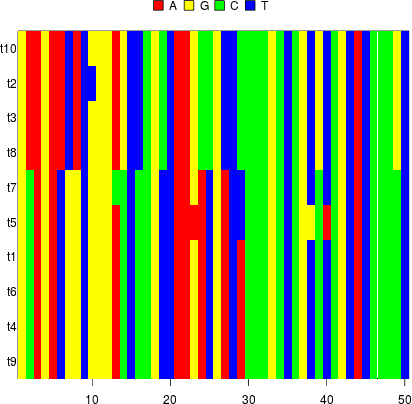
\includegraphics[width=0.2\textwidth]{alignment.png}
    };   
    \node[state] (AL) [above left=-0.25cm and -0.25cm of A, fill=white] {
      1
    };   
    \node[state] (B) [right of = A, rectangle] {
      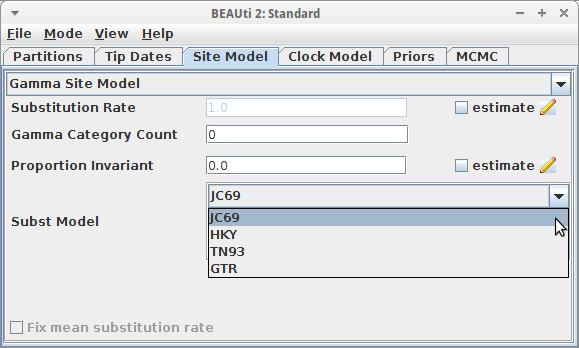
\includegraphics[height=0.15\textheight]{beauti_site_model.png}
    };   
    \node[state] (BL) [above left=-0.25cm and -0.25cm of B, fill=white] {
      2
    };   
    \node[state] (E) [below of=A, rectangle] {
      
\includegraphics[height=0.1\textheight]{file2.png}
    };   
    \node[state] (EL) [above left=-0.25cm and -0.25cm of E, fill=white] {
      3
    };   
    \node[state] (C) [right of = E, rectangle] {
      
\includegraphics[width=0.3\textwidth]{beast_logo.png}
    };   
    \node[state] (CL) [above left=-0.25cm and -0.25cm of C, fill=white] {
      4
    };   
    \node[state] (F) [rectangle, below of=E] {
      
\includegraphics[height=0.1\textheight]{file.png}
    };
    \node[state] (FL) [above left=-0.25cm and -0.25cm of F, fill=white] {
      5
    };   
    \node[state] (H) [rectangle, below of=F] {
      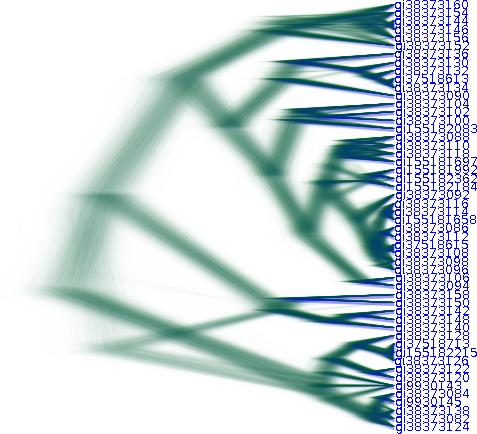
\includegraphics[width=0.3\textwidth]{DensiTreeExample2.jpg}
    };
    \node[state] (HL) [above left=-0.25cm and -0.25cm of H, fill=white] {
      6
    };   
    \node[state] (I) [rectangle, right of=H] {
      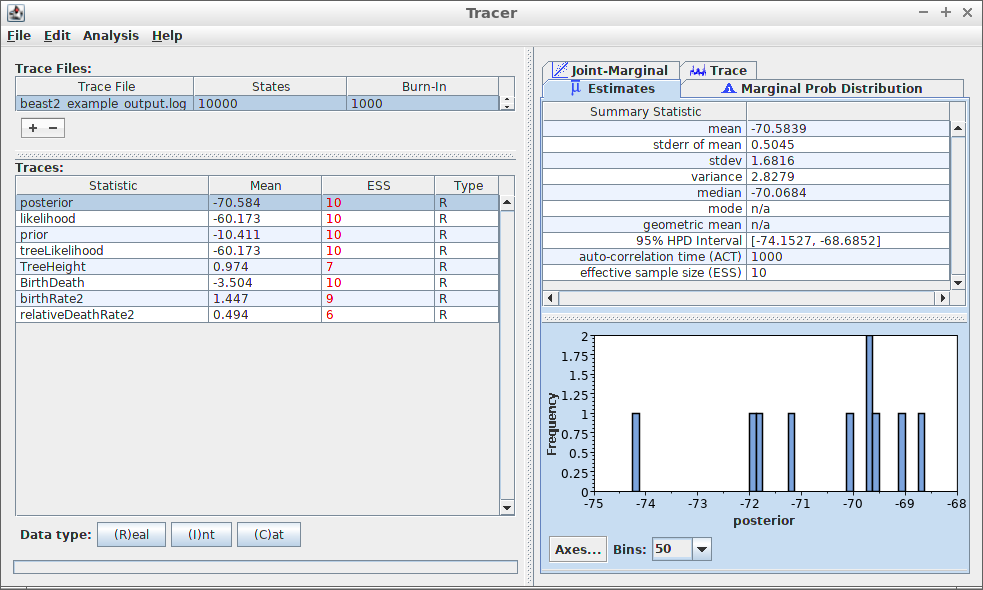
\includegraphics[width=0.6\textwidth]{tracer_example_output.png}
    };
    \node[state] (IL) [above left=-0.25cm and -0.25cm of I, fill=white] {
      7
    };   
    \path 
      (A) edge [anchor = west] node {} (E)
      (E) edge [anchor = west] node {} (F)
      (F) edge [anchor = west] node {} (H)
      (F) edge [anchor = west] node {} (I)
    ; 
    \path [-o,draw] (B) -- ($ (A) !.5! (E) $);
    \path [-o,draw] (C) -- ($ (E) !.5! (F) $);
    \end{tikzpicture}
  }
  \caption{
    Workflow using GUI tools. From an alignment (1) and BEAUti (2), 
    a BEAST2 configuration file (3) is created. BEAST2 (4) uses that file
    to infer a posterior, storing it in multiple files (5). These results
    are visualized using DensiTree (6) and Tracer (7). babette allows
    for the same workflow, all from an R function call.
  }
  \label{fig:workflow}
\end{figure}
%%%%%%%%%%%%%%%%%%%%%%%%%%%%%%%%%%%%%%%%%%%%%%%%%%%%%%%%%%%%%%%%%%%%%%%%%%%%%%%%

\end{document}
